% Options for packages loaded elsewhere
\PassOptionsToPackage{unicode}{hyperref}
\PassOptionsToPackage{hyphens}{url}
\documentclass{beamer}
\usepackage{graphicx}
\usepackage{amsmath}
\usepackage{booktabs}
\usepackage{xcolor}
\usepackage{bookmark}

% Penn colors
\definecolor{pennred}{HTML}{990000}
\definecolor{pennblue}{HTML}{011f5b}

% Beamer theme settings
\usetheme{Madrid}
\setbeamercolor{structure}{fg=pennred}
\setbeamercolor{frametitle}{bg=pennblue, fg=white}
\setbeamercolor{title}{fg=white}
\setbeamercolor{item}{fg=pennred}

\title[Beyond Expected Goals]{Beyond Expected Goals: A Probabilistic Framework for Shot Occurrences in Soccer}
\author[Pipping, Feng, \& Sabin]{Jonathan Pipping, Tianshu Feng, and Paul Sabin}
\date{August 7, 2025}
\institute[UPenn]{University of Pennsylvania}

\begin{document}

\frame{\titlepage}

% What Does It Mean to Deserve a Win?
\begin{frame}[fragile]{What Does It Mean to ``Deserve'' a Win?}
\begin{itemize}
\item \textbf{Match Analysis:} After a match, commentators often remark that a team "didn't deserve the result." But what is this judgment based on?
\item \textbf{Traditional Measure:} Expected Goals (xG), which estimates the quality of shots \emph{taken}. But is that the right metric?
\item \textbf{Our Question:} Which is more notable – getting a shot off, or making it?
\end{itemize}
\end{frame}

% Mbappe Video Example
\begin{frame}{Video Example}
% Video content will be added here
\end{frame}

% What Are Expected Goals (xG)?
\begin{frame}{What Are Expected Goals (xG)?}
\begin{itemize}
\item \textbf{Expected Goals (xG):} a metric that estimates the probability that a shot is scored
\begin{itemize}
  \item Depends on factors like distance from goal, angle to goal, shot type, and player positions
  \item Estimated by XGBoost models trained on historical shot data
\end{itemize}
\item  \textbf{Applications:}
  \begin{itemize}
  \item Estimating the quality of a shot
  \item Measuring of team performance over a match or season
  \item Residualizing provides a measure of shooter skill
  \end{itemize}
\end{itemize}
\end{frame}

% Limitations of xG
\begin{frame}{Limitations of xG}
\begin{itemize}
\item \textbf{Selection Bias:} Models are only trained on \emph{observed} shots
  \begin{itemize}
  \item Skilled attackers take more shots and are more successful on them
  \item Any chance without a recorded shot isn't in the training data
  \end{itemize}
\item \textbf{Aggregation Issues:} An incomplete measure of team performance
\begin{itemize}
  \item Threatening attacks with no recorded shots are omitted
  \item Rebounded chances are double-counted
\end{itemize}
\end{itemize}
\end{frame}

% Visual Examples
\begin{frame}[fragile]{Example 1: No Recorded Shot}
\begin{itemize}
\item \textbf{Match:} Manchester City v Real Madrid (Feb 19, 2025)
\item \textbf{Question:} Which chance was more likely to produce a goal?
\end{itemize}

\vspace{6cm}
% Video will be added here
\end{frame}

% Video Example 2
\begin{frame}{Example 2: $>1$ xG on a Possession}
\begin{itemize}
\item \textbf{Match:} Orlando City vs. Philadelphia Union (February 22, 2025)
\item \textbf{Sequence:} Multiple shots in one possession totaling 1.63 xG
\end{itemize}

\vspace{6cm}
% Video will be added here
\end{frame}

\begin{frame}{Example 2: $>1$ xG on a Possession}
\begin{table}[h]
\centering
\begin{tabular}{|c|l|c|}
\hline
\textbf{Time} & \textbf{Player} & \textbf{Shot Outcome (xG)} \\
\hline
78:01 & Brekalo & Shot Blocked (0.05) \\
78:02 & Muriel & Shot Post (0.52) \\
78:04 & Pasalic & Shot Post (0.68) \\
78:05 & Pasalic & Shot Goal (0.38) \\
\hline
\end{tabular}
\caption{Sequence of shots leading to a goal, totaling 1.63 xG.}
\end{table}
\end{frame}

% Our Target Metric: xG+
\begin{frame}{Our Target Metric: xG+}
\begin{itemize}
\item A more complete picture of goal expectancy
  \begin{itemize}
  \item Accounts for high-threat attacks with no shots
  \item Avoids double-counting rebounded chances
  \end{itemize}
\item At each frame $t$, let xG+ be the probability of a goal:
\begin{align*}
\text{xG+}_t &= \mathbb{P}_t(\text{goal scored}) \\
&= \mathbb{P}_t(\text{goal scored} \mid \text{shot taken})\cdot\mathbb{P}_t(\text{shot taken}) \\
&= \text{xG}_t\cdot\text{xShot}_t
\end{align*}
\item Then define xG+ over a possession with $n$ frames:
$$\text{xG+}_\text{poss} = 1 - \prod_{t = 1}^n \left(1 - \mathbb{P}_t\left(\text{goal scored}\right)\right)$$
\item Estimating this value requires fitting two models: xG and xShot
\end{itemize}
\end{frame}

% Data Overview
\begin{frame}{Data Overview}
\begin{itemize}
\item \textbf{Source:} Gradient Sports (formerly PFF FC) video tracking and event data from the 2022-2025 English Premier League
\item \textbf{Key Features:}
  \begin{itemize}
  \item Player positions (x, y) at 30 frames per second
  \item Ball position (x, y, z) at 30 frames per second
  \item Shot events and outcomes
  \item Team possession indicators
  \item Player and team identifiers
  \end{itemize}
\end{itemize}
\end{frame}

% Data Cleaning
\begin{frame}{Data Cleaning}
\begin{itemize}
\item \textbf{Filtering:} Keep frames where the ball is in play and a team has clear possession
\item \textbf{Smooth Ball Tracking:} Linearly interpolate ball positions to fill in missing frames
\item \textbf{Define Attacking Sequences:}
  \begin{itemize}
  \item Start: team gains possession in their attacking third
  \item End: defending team regains possession or ball exits attacking third
  \end{itemize}
\item \textbf{Field Standardization:} Flip right-to-left attacks $180^{\circ}$ to make all attacks go left-to-right
\end{itemize}
\end{frame}

% Feature Engineering
\begin{frame}{Feature Engineering}
\begin{itemize}
\item \textbf{Ball Features:}
  \begin{itemize}
  \item Distance from goal ($r_{ball}$)
  \item Angle to goal ($\theta_{ball}$)
  \item Ball height ($z_{ball}$)
  \item Ball speed ($v_{ball}$)
  \end{itemize}
\item \textbf{Player Features:}
  \begin{itemize}
  \item Position of 5 closest offensive teammates relative to the ball ($r_{off}, \theta_{off}$)
  \item Position of 5 closest non-GK defenders relative to the ball ($r_{def}, \theta_{def}$)
  \item Position of goalkeeper relative to the goal ($r_{gk}, \theta_{gk}$)
  \end{itemize}
\item \textbf{Goal Openness:}
  \begin{itemize}
    \item Model defenders as circles with diameter 0.75m
    \item Draw tangent lines from the ball to defenders and find where they meet the goal line
    \item Call the percentage of the goal that's unobstructed \texttt{openGoal}
  \end{itemize}
\end{itemize}
\end{frame}

% Modeling
\begin{frame}{Modeling}
\begin{itemize}
\item \textbf{Training Data:} All data from the 2022-2025 Premier League seasons
\item \textbf{Features:} Ball features, player features, and goal openness
\item \textbf{Models:}
  \begin{itemize}
  \item \textbf{xG:} 5-fold cross-validated XGBoost model estimating the probability that a shot is scored
\item \textbf{xShot:} 5-fold cross-validated XGBoost model estimating the probability that a shot occurs \emph{in the next second}
  \end{itemize}
\item \textbf{Evaluation Metric:} Log loss
\end{itemize}
\end{frame}

% Results - xG model
\begin{frame}{xG Model Results}
\begin{columns}[c]
  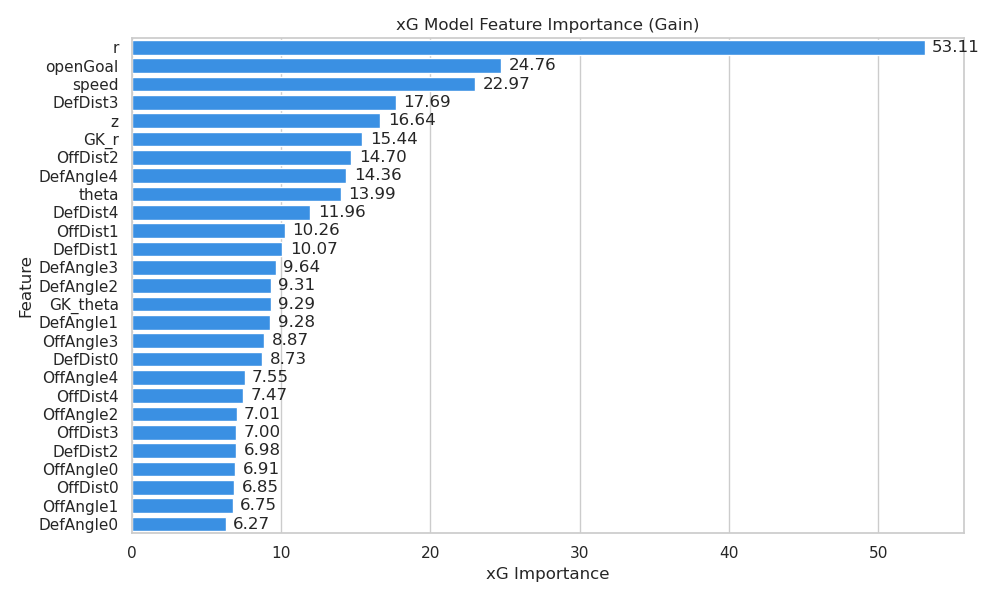
\includegraphics[width=\linewidth]{figures/xG_feature_importance.png}
\end{columns}
\end{frame}

\begin{frame}{xG Model Results}
\begin{columns}[c]
  \column{0.4\textwidth}
  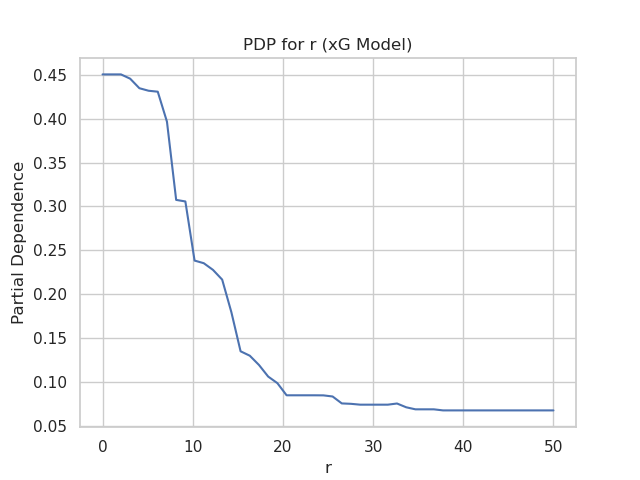
\includegraphics[width=\linewidth]{figures/xG_PDP_r.png}
  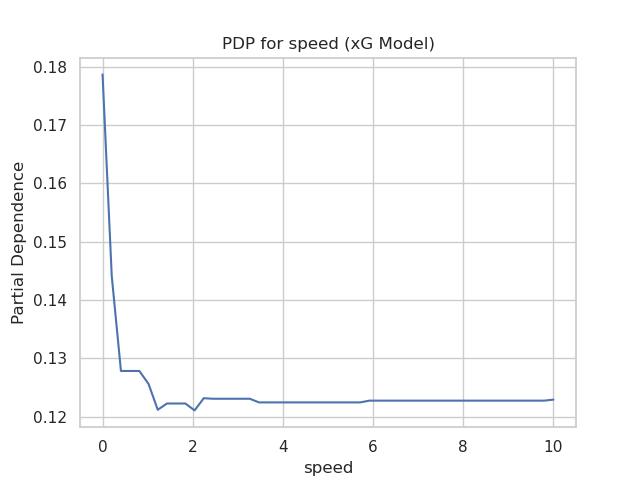
\includegraphics[width=\linewidth]{figures/xG_PDP_speed.png}

  \column{0.4\textwidth}
  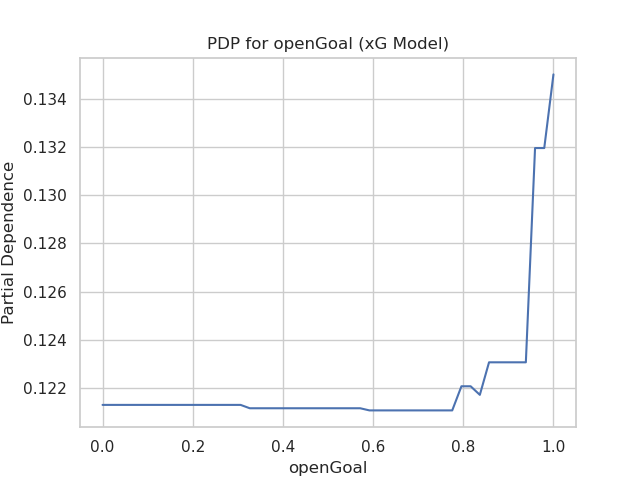
\includegraphics[width=\linewidth]{figures/xG_PDP_openGoal.png}
  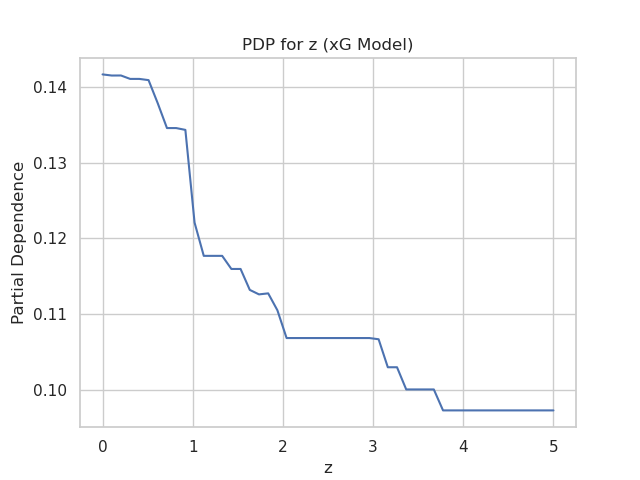
\includegraphics[width=\linewidth]{figures/xG_PDP_z.png}
\end{columns}
\end{frame}

% Results - xShot model
\begin{frame}{xS Model Results}
\begin{columns}[c]
  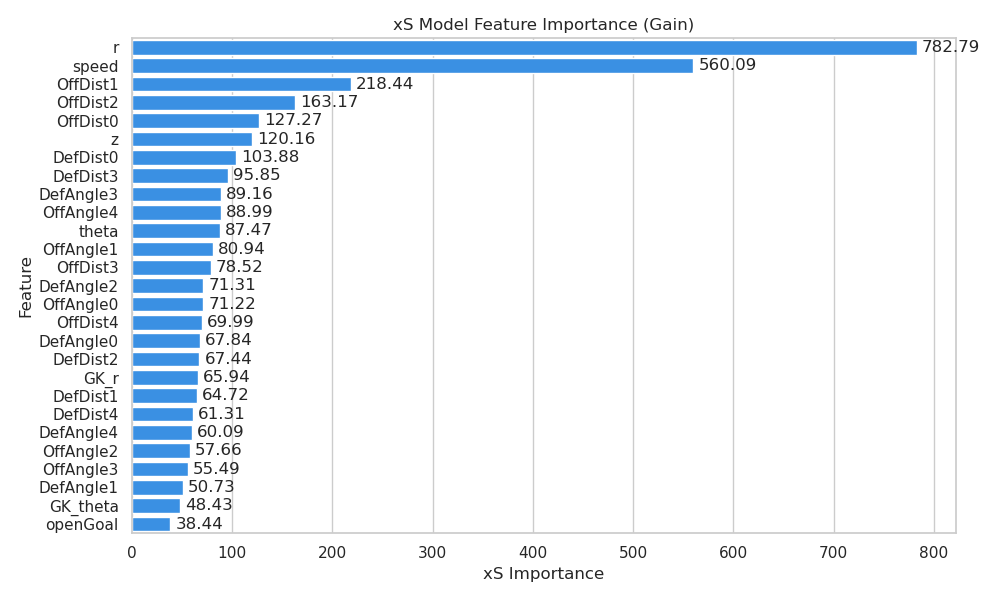
\includegraphics[width=\linewidth]{figures/xS_feature_importance.png}
\end{columns}
\end{frame}

\begin{frame}{xS Model Results}
\begin{columns}[c]
  \column{0.5\textwidth}
  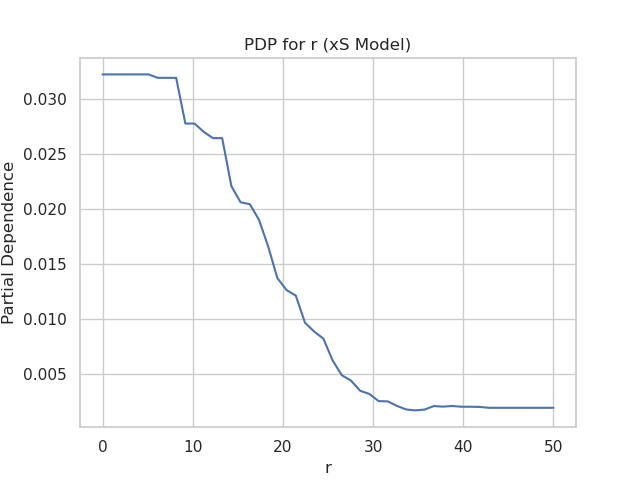
\includegraphics[width=\linewidth]{figures/xS_PDP_r.png}

  \column{0.5\textwidth}
  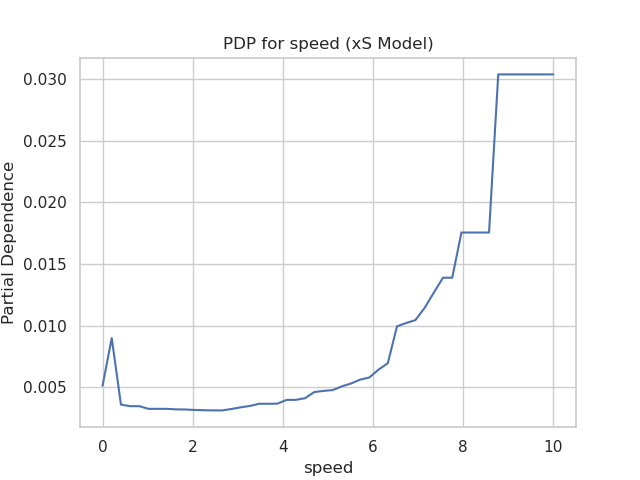
\includegraphics[width=\linewidth]{figures/xS_PDP_speed.png}
\end{columns}
\end{frame}

% Cross-Validation Study
\begin{frame}{Cross-Validation Study}
\begin{itemize}
\item \textbf{Objective:} Evaluate xG+ performance using cross-validated Poisson models
\item \textbf{Dataset:} 3 seasons of EPL match data
\item \textbf{Method:} Train on all matchdays except one, predict goals on held-out data
\item \textbf{Goal:} Determine how well adjusted xG+ explains actual goals scored
\end{itemize}
\end{frame}

% Cross-Validation Setup
\begin{frame}{Cross-Validation Setup}
\begin{itemize}
\item \textbf{Setup:} Treat each matchday as a fold.
$$38 \text{ matchdays} \times 3 \text{ seasons} = 114 \text{ folds}$$
\item \textbf{For each fold:}
  \begin{itemize}
  \item Train on all matchdays except one to acquire adjusted metrics
  \item Poisson regression on team goals using training data
  \item Predict goals scored on held-out matchday test data
  \end{itemize}
\end{itemize}
\end{frame}

% Metrics and Aggregation Methods
\begin{frame}{Metrics and Aggregation Methods}
\textbf{Metrics:}
\begin{itemize}
\item \textbf{xS:} Probability a player takes a shot in the next second
\item \textbf{xG:} Probability that a shot is scored
\item \textbf{xG+:} xS $\times$ xG, the probability of scoring in the next second
\end{itemize}

\textbf{Aggregation Methods:}
\begin{enumerate}
\item \textbf{Max-per-possession:} Take maximum 1-second prediction in each possession
\item \textbf{At-least-one-per-possession:} $1 - \prod (1 - p)$ across possession
\item \textbf{Sum-of-shots:} Traditional xG summed over actual shots
\end{enumerate}
\end{frame}

% Mixed Effects Modeling
\begin{frame}{Mixed Effects Modeling}
\textbf{Fitted on training data for each fold:}
$$\texttt{metric} \sim (1|\texttt{season}) + (1|\texttt{season:team}) + (1|\texttt{season:opp}) + \texttt{home}$$

\textbf{Extracted Effects:}
\begin{itemize}
\item Team attack (per season)
\item Opponent defense (per season)
\item Season effect
\item Home field advantage
\end{itemize}
\end{frame}

% Secondary Poisson Model
\begin{frame}{Secondary Poisson Model}
\textbf{Train Poisson regression on adjusted metrics:}
$$\texttt{goals} \sim \texttt{home} + \texttt{season} + \texttt{team\_off} + \texttt{opp\_def}$$

\textbf{Purpose:} Assess predictive utility of each adjusted metric on actual goals
\end{frame}

% Cross-Validation Results
\begin{frame}{Cross-Validation Results}
\begin{table}[!h]
\centering
\caption{Mean Squared Error (MSE) by Metric and Aggregation Method}
\begin{tabular}[t]{lrrr}
\toprule
Aggregation Method & xG+ & xS & xG\\
\midrule
At-least-one-per-possession & 2.84 & 2.90 & 2.94\\
Max-per-possession & 2.84 & 2.87 & 2.91\\
Sum-of-shots &  &  & 2.90\\
\bottomrule
\end{tabular}
\end{table}
\end{frame}

\begin{frame}{Cross-Validation Results}
\begin{table}[!h]
\centering
\caption{Mean Absolute Error (MAE) by Metric and Aggregation Method}
\begin{tabular}[t]{lrrr}
\toprule
Aggregation Method & xG+ & xS & xG\\
\midrule
At-least-one-per-possession & 1.86 & 1.87 & 1.89\\
Max-per-possession & 1.86 & 1.86 & 1.89\\
Sum-of-shots &  &  & 1.87\\
\bottomrule
\end{tabular}
\end{table}
\end{frame}

% Player Ability
\begin{frame}{Player Ability}
\begin{itemize}
\item \textbf{Question:} Does this framework provide insight into individual player skills?
\item \textbf{Methodology:}
  \begin{itemize}
  \item Aggregate chances for the closest player to the ball within a possession
  \item Sum up per game \& season for each of xG, xS, and xG+
  \item Compare actual shots \& goals to expected metrics
  \item Analyze year-over-year performance consistency
  \end{itemize}
\item \textbf{Key Finding:} Players \emph{do not} consistently over-perform their expected goals (xG)
\end{itemize}
\end{frame}

\begin{frame}{Player Ability}
\begin{itemize}
\item \textbf{Key Finding:} Players \emph{do} consistently over-perform as shot takers!
\item \textbf{Implication:} Generally, elite goal scorers are the ones converting chances into shots, not converting shots into goals!
\end{itemize}

\begin{table}[!h]
\centering
\caption{Year to Year Correlation (Stability) vs. Expected (Per Game)}
\begin{tabular}[t]{rrr}
\toprule
xG & xS & xG+\\
\midrule
0.12 & 0.63 & 0.35\\
\bottomrule
\end{tabular}
\end{table}
\end{frame}

% Results
\begin{frame}{Player Ability}
\begin{itemize}
\item \textbf{Example:} Haaland's record breaking season (36 goals)
\item \textbf{Key Insight:} Required both higher shots and goals than expected
\end{itemize}

\centering
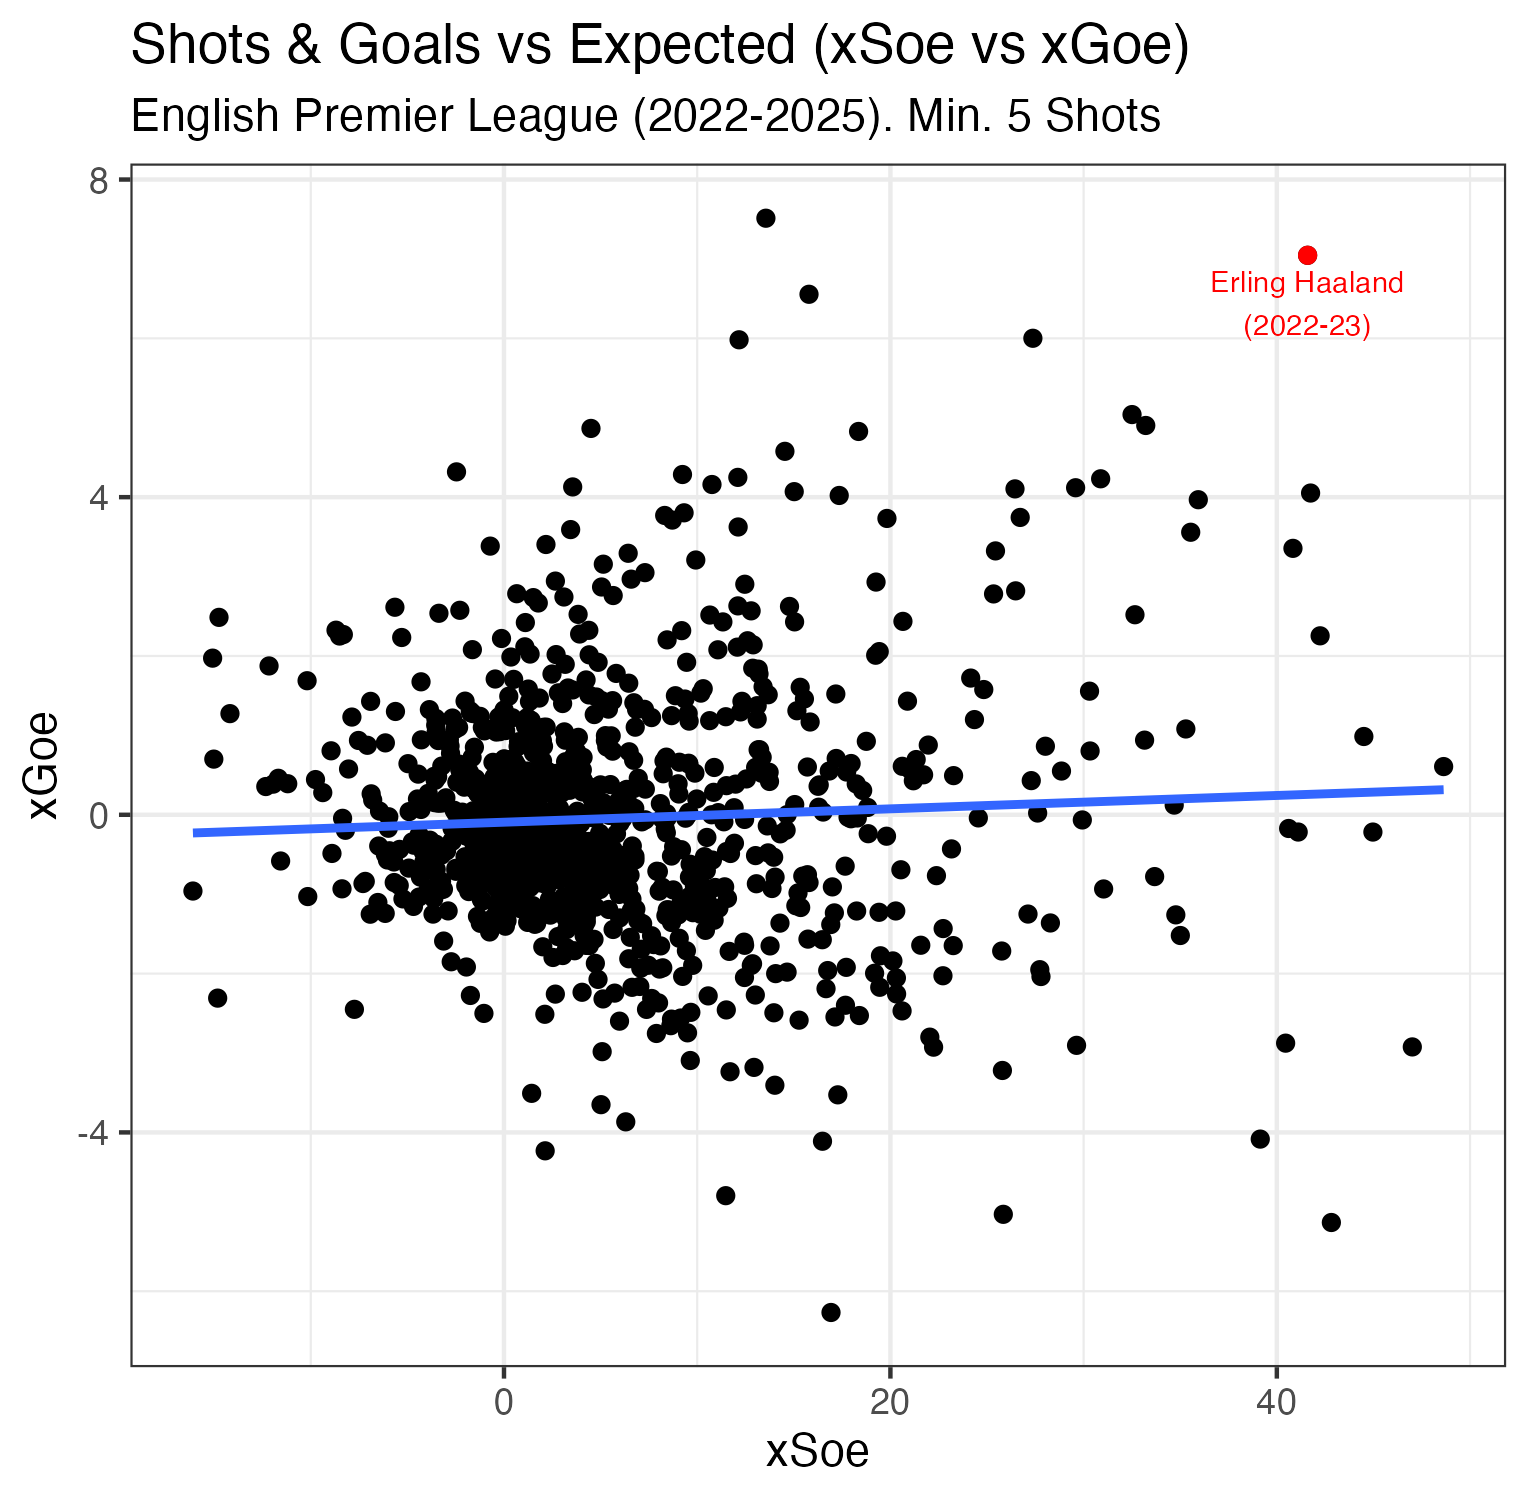
\includegraphics[width=2.75in]{figures/xseoe_vs_xgoe.png}
\end{frame}

\begin{frame}{Top Over-Expectation Performers (Per Game)}
\tiny
\centering
\textbf{xG+ Over Expected} \\
\vspace{0.1cm}
\begin{tabular}{llrrrrr}
\toprule
\textbf{Season} & \textbf{Player} & \textbf{xG+ OE} & \textbf{Goals} & \textbf{Games} & \textbf{Chances} \\
\midrule
2022--23 & Erling Haaland     & 0.52 & 36 & 35 & 444 \\
2023--24 & Erling Haaland     & 0.44 & 30 & 31 & 513 \\
2024--25 & Omar Marmoush      & 0.41 & 10 & 16 & 293 \\
2024--25 & Yoane Wissa        & 0.35 & 22 & 35 & 429 \\
2024--25 & Mohamed Salah      & 0.33 & 27 & 38 &1042 \\
2024--25 & Chris Wood         & 0.31 & 23 & 36 & 330 \\
2023--24 & Cole Palmer        & 0.30 & 19 & 34 & 693 \\
2024--25 & Alexander Isak     & 0.30 & 25 & 34 & 558 \\
2023--24 & Alexander Isak     & 0.30 & 19 & 28 & 351 \\
2022--23 & Harry Kane         & 0.29 & 25 & 38 & 589 \\
\bottomrule
\end{tabular}

\vspace{0.25cm}
\textbf{xG Over Expected} \\
\vspace{0.1cm}
\begin{tabular}{llrrrrr}
\toprule
\textbf{Season} & \textbf{Player} & \textbf{xG OE} & \textbf{Goals} & \textbf{Games} & \textbf{Chances} \\
\midrule
2024--25 & Omar Marmoush      & 0.41 & 10 & 16 & 293 \\
2024--25 & Chris Wood         & 0.31 & 23 & 36 & 330 \\
2024--25 & Michael Keane      & 0.21 &  3 & 10 &  19 \\
2022--23 & Erling Haaland     & 0.52 & 36 & 35 & 444 \\
2022--23 & Roberto Firmino    & 0.25 & 10 & 21 & 253 \\
2022--23 & Martin Ödegaard    & 0.22 & 15 & 37 & 942 \\
2023--24 & Heung-min Son      & 0.28 & 20 & 35 & 751 \\
2022--23 & Matias Viña        & 0.26 &  3 & 10 &  66 \\
2022--23 & Alexander Isak     & 0.24 & 11 & 22 & 346 \\
2023--24 & Taiwo Awoniyi      & 0.26 &  7 & 19 & 125 \\
\bottomrule
\end{tabular}

\vspace{0.1cm}
\emph{Note: Minimum 10 Games with a Chance}
\end{frame}

% Conclusions
\begin{frame}{Conclusions}
\begin{itemize}
\item \textbf{Best Metric for Team Prediction:} xG+
\item \textbf{Best Aggregation Method:} At-least-one-per-possession
\item \textbf{Player Evaluation:} Shots over expected is more predictive of future player performance than goals over xG
\item \textbf{Future Work:} An instantaneous or time-weighted xShot model
\item \textbf{Questions and Discussion}
\end{itemize}
\end{frame}

% Acknowledgements
\begin{frame}{Acknowledgements}
\begin{itemize}
\item Special thanks to our data providers at Gradient Sports (formerly PFF FC)
\item All work supported by the Wharton Sports Analytics \& Business Initiative (WSABI)
\end{itemize}
\end{frame}

\end{document}